\section{Advanced IR}
\subsection{Latent semantic indexing}

Vector space retrieval is vague and noisy
\begin{itemize}
\item Based on index terms
\item Unrelated documents might be included in the answer set
\item Relevant documents that do not contain at least one index term
  are not retrieved
\item \textbf{Observation} user information needs are more related to
  concepts than to index terms
\end{itemize}

\subsubsection{The problem}
Vector space retrieval handles poorly the following two conditions:
\textit{Synonymy} (poor recall) and \textit{Homonymy}(poor precision).

\subsubsection{Key Idea}
Map documents and queries into a lower-dimensional space composed of
higher level concepts.
\begin{itemize}
\item Each concept represented by a combination of terms
\item Fewer concepts than terms
\item \textbf{Vehicle} = [car, automobile, wheels, autocar, motor car]
\end{itemize}

\subsubsection{Similarity computation in concept space}
Concept represented by terms, e.g.\: device = {iOS, iPad, mobile}
Document represented by concept vector which contians number of
occurences of words grouped by concept. \textbf{Similarity} is the
scalar product of normalized concept vectors.

\subsubsection{Basic definitions}
How to identify and compute ``concepts''? \\
Consider the term document matrix
\begin{itemize}
\item Let $ M_{ij} $ be a term document matrix with m rows (terms) and
  n columns (documents). \textbf{Reverse of classic vector space}!
\item To each element of this matrix is assigned a weight $ w_{ij} $
  associated with $ t_i $ and $ d_j $
\item The weight $ w_{ij} $ can be based on a tf-idf weighting scheme
\item The ranking is then the result of computing the product of the
  term-document matrix with the query vector, assuming that all
  columns in M and q are normalized to 1
\end{itemize}

\subsubsection{Singular value decomposition}
Represent matrix M as $ M = K S D^t $
\begin{itemize}
\item K and D are matrices with orthonormal columns: $ K K^t = I = D
  D^t $
\item S is an $ r \times r $ diagonal matrix of the singular values
  sorted in decreasing order where $ r = min(m, n) $, the rank of M
\item Such a decomposition is unique and always exists (up to sign)
\end{itemize}

Construction of SVD
\begin{itemize}
\item K is the matrix of eigenvectors derived from $ M M^t $
\item D is the matrix of eigenvectors derived from $ M^t M $
\item S is a diagonal matrix with the eigenvalues in the diagonal
\end{itemize}

We can write M as sum of outer vector products

$ M = \sum_{i = 1}^r s_i k_i \oplus d'_i $

The $ s_i $ are ordered in decreasing size.
By taking only the largets ones we obtain a good approximation of M
(LSE). The singular values $ s_i $ are the lengths of the semi axes of
the hyperellipsoid E defined by $ E = \big\{ Mx \mid \| x |_2 = 1
  \big\} $ \\

In the matrix S select only the $ s $ largest singular values and keep
the corresponding columns in K and D.
The resultat matrix, $ M_s $ is given by $ M_s = K_s S_s D_s^t $ where
s, $ s < r $, is the dim of the concept space.

The parameter s should be large enough to allow fitting the
characteristic of the data and small enough to filter out non relevant
representational details.

\subsubsection{Answering queries}

Documents are compared by computing cosine similarity in concept
space, i.e.\ , comparing theire columns $ (D_s^t)_i $ and $ (D_s^t)_j
$ in matrix $ D_s^t $.

A query q is treated like one more document
\begin{itemize}
\item it is added as an additional column to M
\item the same transformation is applied as for mapping M  to D
\end{itemize}

\subsubsection{Mapping queries}

Mapping of M to D
\begin{align*}
  &M = K S D^t
  &S^{-1} K^t M = D^t \text{since }KK^t = 1
  &D = M^t K S^{-1}
\end{align*}

Apply the same transformation to q
$ q^* = q^t K_s S_s^{-1} $

Then compare transformed vector by standard cosine similarity
$ sim(q^*, d_i) = \frac{q^* \cdot (D_s^t)_i}{\mid q^* \mid \mid
  (D_s^t)_i \mid}  $

\subsubsection{Discussion}

Advantages
\begin{itemize}
\item Allows reducing the complexity of the underlygin concept repr
\item Facilitates interfacing with user
\end{itemize}

\begin{itemize}
\item Computationaly expensive
\item Poor statistical explanation
\end{itemize}

\subsection{Alternative techniques}

Probabilistic latent semantic analysis (bayesian networks) \\

Latent dirichlet allocation:
\begin{itemize}
\item Based on dirichlet distribution
\item state of the art method for concept extraction
\end{itemize}

Same objective creating a concept space based on the term-document
matrix
\begin{itemize}
\item better explained math foundation
\item better experimental results
\end{itemize}

\subsubsection{Latent dirichlet allocation}

\textbf{Idea}: assume a document collection is randomly generated from
a know set of topics (prob generative model). \\

\textbf{Document generation} \\
\begin{itemize}
\item For each document, choose a mixture of topics
\item For every word position sample a topic [1,\ldots, T] from the
  topic mixture
\item For every word position sample a word from the chosen topic
\end{itemize}

\subsubsection{LDA: Topic identification}
Inverting the process: given a document collection, reconstruct the
topic model.
\begin{itemize}
\item Topics are \textbf{interpretable} unlink arbitrary dimensions of
  LSI
\item Distributions follow a Dirichlet distribution
\item Construction of topic is feasible
\item State-of-the-art method for topic id
\end{itemize}

\subsubsection{Use of topic models}

\texttt{Unsupervised learning} of topics
\begin{itemize}
\item Understanding main topics of a topic colllection
\item Organizing the document collection
\end{itemize}

Document retrieval: use topic vectors  instead of term vectors in
representations.

Document classification (\texttt{supervised learning}): use topics as
features.

\section{Word embeddings}

\subsection{Word context}

The neighborhood of a word expresses a lot about is meaning.
\begin{itemize}
\item Word: w = banking
\item Context: C(w) = \{government, debt, problems, crises, \ldots\}
\item Word-context occurence: $ (w, c)\,, c \in C(w) $
\end{itemize}

\subsection{Similarity based representation}
\begin{itemize}
\item Two words are considered as similar, when they have similar
  context
\item Context captures both syntactic and semantic similary
  (\textbf{syntactic}: king - kings, \textbf{semantic}: king - queen)
\item Implicitly used in the term-document matrix
  \begin{itemize}
  \item less localized content
  \item No distinction between context and word
  \end{itemize}
\end{itemize}

\textbf{Idea}: try to model how likely a word and a context occur
together.
\begin{itemize}
\item Map words into a low-dimensional space (d=200)
\item Map context words into the same low-dimensional space, different
  mapping for same words!
\item Interpret the vector distance (product) as a measure for how
  likely the word and its context occur together
\item Due to projection in low-dim space, similar words and contexts
  should be close
\end{itemize}

\subsection{Learning the model from the data}
Consider a pair $ (w, c) $ \\
Probability that it originates from the data: \\
$ p(D = 1 \mid w,c;\theta) = \frac{1}{1 + e^{-v_c \cdot v_w }} =
\sigma(v_c \cdot v_w) $

This is a binary classification problem solved by logistic
regression.

\subsubsection{Adding negative samples}

Considering positives samples $ (w, c) $ as well as negative samples
(not occuring in the document collection). Find $ \theta $ s.t.\ the
overall probability is maximized:
$ \theta = argmax_\theta \prod_{(w,c) \in D} P(D = 1 \mid w,c,\theta)
\prod_{(w,c) \in \neg{D}} P(D = 0 \mid w,c,\theta) $

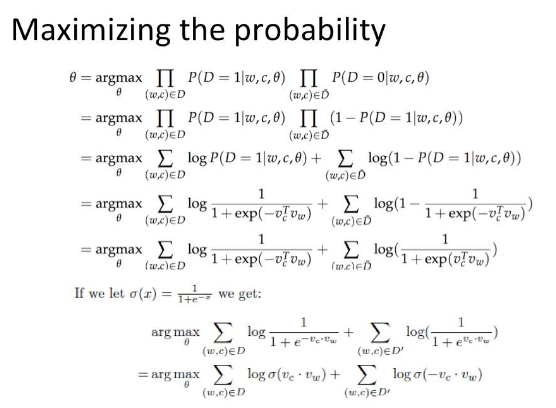
\includegraphics[width=220px,height=150px]{negsample}

\subsection{Stochastic gradient descent}

Define a loss function $ J(\theta) = - log(\sigma(v_c \cdot v_w)) -
\sum_{k=1}^K log(\sigma(v_{c_k} \cdot v_w)) $ \\
For every (w, c) in D, update $ \theta $: \\
$ \theta^{new} = \theta^{old} - \alpha \nabla_{theta} J_t(\theta) $

Updates only affect rows in $ W^{(1)} $ and $ W^{(2)} $ where c and w
appear.

\subsubsection{Obtaining negative samples}
Negatives samples are taken from $ P_n(w) = V \setminus C(w) $ \\
Empirical approach
\begin{itemize}
\item If $ p_w $ is the probability of word w in collection, choose
  with probability $ p_w^{3/4} $
\item Less frequent words are sampled more often
\item approximate the probability by sampling a few non-context words
\end{itemize}

\subsubsection{Result}
Matrices $ W^{(1)} $ and $ W^{(2)} $ that captures information on word
similarity
\begin{itemize}
\item Words appearing in similar contexts generate similar contexts
  and vice-versa
\item Hence, mapped to similar representations in lower dimensional
  space
\item Use $ W = W^{(1)} + W^{(2)} $ as low-dimensional representation
\end{itemize}

\subsection{Properties of word embeddings}
\begin{itemize}
\item Similar terms are clustered
\item Syntactic and semantic relationships encoded as linear mappings
\item Dimensions can capture meanings
\end{itemize}

\subsection{Use of word embeddings models}
Thesaurus construction and taxonomy induction. \\
Document classification.

%%% Local Variables:
%%% mode: latex
%%% TeX-master: "master"
%%% End:
